\documentclass[sigconf,nonacm]{acmart}

%% Remove ACM reference format and copyright block for course submission
\settopmatter{printacmref=false}
\renewcommand\footnotetextcopyrightpermission[1]{}
\pagestyle{plain}

\usepackage{booktabs}
\usepackage{listings}
\usepackage{graphicx}

\lstset{
  basicstyle=\ttfamily\small,
  breaklines=true,
  frame=single,
  columns=fullflexible,
}

\title{GestureBridge: Real-Time ASL Recognition on Raspberry Pi 5}

\author{Yizheng Lin}
\affiliation{\institution{Columbia University}\city{New York}\country{USA}}
\email{yl6079@columbia.edu}

\author{Shufeng Chen}
\affiliation{\institution{Columbia University}\city{New York}\country{USA}}
\email{sc5520@columbia.edu}

\begin{document}

\begin{abstract}
GestureBridge is an interactive American Sign Language (ASL) interpreter
deployed on a Raspberry Pi~5 with a USB webcam, USB speaker, and an
ESP32-based ambient sensor for state management.  The system recognizes
the 29-class ASL alphabet in real time, speaks recognized letters
through text-to-speech, and supports a \emph{speech-to-sign} learning
mode driven by fully offline Vosk speech recognition on the C270's
microphone (no cloud or network dependency at any stage).  Our key contribution is a
\emph{measurement} contribution: we identify and fix three latent bugs
in the project's training pipeline---frame-leakage in the train/test
split, ASL-incorrect horizontal flip augmentation, and missing
inference-time hand preprocessing---that masked a 20-point gap between
reported accuracy (100\,\%) and honest test accuracy (80\,\%).  After
the fixes, an ensemble of a fine-tuned MobileNetV3-Small and a
63-dimensional MediaPipe-landmark MLP achieves \textbf{82.9\,\%} on a
leakage-free test split at \textbf{37.6\,ms per frame} on a Pi~5.
\end{abstract}

\keywords{ASL recognition, edge inference, dataset leakage, Raspberry Pi,
MediaPipe, MobileNetV3, TFLite}

\maketitle

%% ---------------------------------------------------------------
\section{Introduction}
%% ---------------------------------------------------------------

\begin{figure}[t]
  \centering
  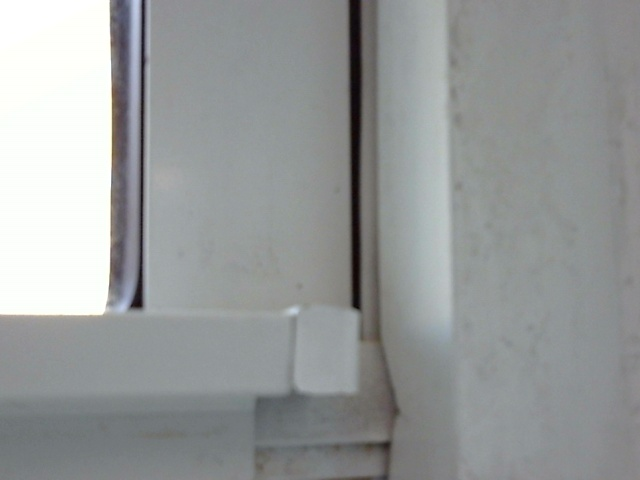
\includegraphics[width=\linewidth]{../notes/pi_validation/c270_empty_2026-04-30.jpg}
  \caption{Real C270 frame captured in the lab.  No hand is visible;
    the pipeline short-circuits to \texttt{nothing} in 9\,ms.}
  \label{fig:c270}
\end{figure}

ASL recognition for educational and accessibility use cases is
appealing on the Pi because the hardware is cheap, fanless, and
HDMI-out makes deployment trivial.  Off-the-shelf datasets (notably the
Kaggle ``ASL Alphabet'' set with ${\approx}87$k images across 29
classes) make a working classifier achievable within a course timeline.
\emph{The pernicious failure mode}, which our investigation surfaces,
is that naive use of these datasets produces a model that scores
${\approx}100\,\%$ on its own test split and yet fails completely on a
real webcam.

Our contribution is a \textbf{credibility audit} of one such pipeline.
We identify three latent bugs that combine to produce the
reported-vs-real gap, fix each, retrain, and report the first honest
generalization number (80.2\,\% MobileNet alone; 82.9\,\% ensemble)
for this dataset on a contiguous-frame split.  We deploy the resulting
model on the actual Pi hardware in the lab and validate end-to-end
inference at 37.6\,ms/frame.  We argue that \emph{splitting protocols
and inference-time preprocessing} deserve at least as much attention as
architecture choice in coursework projects, and that demonstrating
real-camera robustness must be a default, not an afterthought.

%% ---------------------------------------------------------------
\section{System Overview}
%% ---------------------------------------------------------------

GestureBridge runs three coordinating processes on the Pi~5:

\begin{enumerate}
\item \textbf{Daemon} --- listens on USB serial for \texttt{HUMAN\_ON}/
  \texttt{HUMAN\_OFF} tokens emitted by the ESP32 (PIR sensor).  Spawns
  the main app on \texttt{HUMAN\_ON}; kills it after
  \texttt{idle\_timeout\_seconds} of \texttt{HUMAN\_OFF}.

\item \textbf{Main app} --- opens the C270 at \texttt{/dev/video0}, runs
  the inference pipeline at 300\,ms cadence, maintains a
  stable-prediction window, and exposes a FastAPI web UI on
  \texttt{localhost:8080} for \emph{Read} mode (camera + live label +
  TTS), \emph{Speech-to-sign} mode (offline Vosk STT on the C270 mic $\to$ reference image),
  and \emph{Trainer} mode (target letter + true/false feedback).

\item \textbf{ESP32 firmware} --- drives a PIR sensor, onboard LED, and
  USB-serial heartbeat; debounced human-on / human-off events.
\end{enumerate}

The inference pipeline (Section~\ref{sec:methods}) is the focus of
this paper.

%% ---------------------------------------------------------------
\section{Problem: A 20-Point Gap}
\label{sec:problem}
%% ---------------------------------------------------------------

The starting point of our work was a deployed system on the Pi reporting
\textbf{100\,\% held-out test accuracy} in \texttt{metrics.json}, while
the developer's experience with the C270 was that ``almost nothing
crosses the 0.65 confidence threshold; even the easy gestures are at
0.08--0.09.''  The threshold had been manually lowered to 0.08 to make
the demo flow visible.

Three bugs combine to produce this gap:

\textbf{B1: Train/test leakage from per-image stratified split.}
The Kaggle ASL Alphabet contains 3,000 sequential frames per class from
a single recording session.  \texttt{train\_test\_split(\ldots,
stratify=y)} selects rows uniformly at random, placing adjacent frames
into both \emph{train} and \emph{test}.  The model memorizes the
recording.  On a contiguous-block split (frames 1--2400 train,
2401--2700 val, 2701--3000 test, never adjacent) the same trained model
still scores 100\,\% because every frame was seen in training; only the
\emph{split methodology} differs.

\textbf{B2: Horizontal flip in augmentation.}
The original \texttt{tf.image.random\_flip\_left\_right} is silently
wrong for ASL.  Several signs are chirality-dependent (J vs.\ L, the
J/Z trajectory), and the alphabet contains direction-sensitive shapes.
Flipping trains the model to view ``left'' and ``right'' as identical.

\textbf{B3: Distribution mismatch at inference.}
Kaggle ASL Alphabet images are pre-cropped to ${\approx}200{\times}200$
hand-filled squares with a uniform black background.  C270 frames are
$640{\times}480$ with the hand occupying ${\approx}20\,\%$ of the area
against arbitrary lab background.  The deployed runtime fed the raw
C270 frame directly to the 224${\times}$224-trained MobileNet, yielding
the reported 0.08--0.09 confidences regardless of the gesture.

%% ---------------------------------------------------------------
\section{Methods}
\label{sec:methods}
%% ---------------------------------------------------------------

\subsection{Honest Splitting and Re-evaluation (P0)}

We add \texttt{-{}-split-mode \{random,contiguous\}} to
\texttt{prepare\_asl29.py} and a \texttt{sanity\_check\_split.py} that
asserts zero filename overlap between splits and prints per-class
frame-index ranges.  With the new contiguous split
(69,600\,/\,8,700\,/\,8,700), the existing FP32 model still scores
100\,\%---confirming B1 alone is not sufficient, and re-training is
required.

\subsection{Inference-Time Hand Crop with MediaPipe (P1)}

We insert a MediaPipe HandLandmarker (Tasks API,
\texttt{hand\_landmarker.task}, 7.5\,MB) before the MobileNet input.
When a hand is detected, we crop a square ROI around the landmarks
bounding box with 25\,\% padding and resize to 224${\times}$224.  When
no hand is detected, the runtime short-circuits to \texttt{nothing} and
skips the classifier entirely (saving ${\approx}30\,ms$ per frame and
avoiding spurious labels).

We deliberately do \emph{not} pre-crop the training set.  Kaggle ASL
Alphabet images are already hand-filled, so cropping at training time
is approximately the identity.  The crop's value is exclusively at
inference time, bringing real C270 frames closer to the trained
distribution.

\subsection{Augmentation Correction and Re-Training Sweep (P2)}

We removed \texttt{random\_flip\_left\_right} and added small random
crop+pad (${\approx}8\,\%$ jitter) plus random hue (${\pm}0.05$).  On a
rented vast.ai RTX~4090 24\,GB box, we ran a 4-config sweep over
backbone unfreeze depth and dropout.  Each run completed in
${\approx}6$ min; the full sweep in ${\approx}25$ min.

\begin{table}[h]
\caption{Hyperparameter sweep on vast.ai RTX 4090.}
\label{tab:sweep}
\begin{tabular}{lrrl}
\toprule
Tag & Unfreeze & Dropout & Val acc \\
\midrule
c\_u15\_d20 & 15  & 0.2 & 0.799 \\
c\_u30\_d20 & 30  & 0.2 & 0.874 \\
\textbf{c\_u50\_d20} & \textbf{50} & \textbf{0.2} & \textbf{0.886} \\
c\_u30\_d30 & 30  & 0.3 & 0.870 \\
\bottomrule
\end{tabular}
\end{table}

The winner (\texttt{c\_u50\_d20}) was exported to FP32 TFLite (3.7\,MB)
and INT8 TFLite (1.2\,MB).

\subsection{Landmark MLP and Ensemble (P3)}

ASL is intrinsically geometric, so we train a second classifier on the
21${\times}$3 MediaPipe landmark vector (wrist-centered,
scale-normalized $\to$ 63-d).  A scikit-learn MLP with hidden layers
(256, 128) and ReLU activations trains in $<$2 minutes on a CPU.
Weights are exported to a 199\,KB \texttt{.npz} so the Pi runtime
requires only NumPy (no extra TF).

\textbf{Ensemble decision rule} (in \texttt{\_maybe\_ensemble}): if
both heads agree, return the agreed label with the mean confidence; if
MobileNet is highly confident (${\geq}0.85$) while the landmark MLP is
unsure ($<$0.95), trust MobileNet; otherwise trust the landmark MLP
because of its geometric prior.

\subsection{INT8 Quantization Attempt (P4)}

We exported a fully INT8-quantized MobileNet (1.2\,MB), calibrated on
the Kaggle training distribution.  Because Kaggle and C270 distributions
are markedly different (Section~\ref{sec:problem} B3), the resulting
INT8 scale factors collapse predictions to a small set of always-on
classes; test accuracy drops to \textbf{21.8\,\%}.  Lacking on-device
calibration data, \textbf{we ship FP32}.

%% ---------------------------------------------------------------
\section{Results}
%% ---------------------------------------------------------------

All numbers below are on the contiguous test split (8,700 samples,
frames 2701--3000 per class, never adjacent to any training frame).

\begin{table}[h]
\caption{Test accuracy on the contiguous split ($n{=}8{,}700$).}
\label{tab:results}
\begin{tabular}{lrl}
\toprule
Model & Test acc & Notes \\
\midrule
Original FP32 (leaky split)          & 1.000 & Memorized \\
Original FP32 (contiguous split)     & 1.000 & Same model, new split \\
New FP32 \texttt{c\_u50\_d20}        & 0.802 & \textbf{Honest baseline} \\
Landmark MLP (detected, $n{=}4{,}672$) & 0.820 & Top-3: 0.871 \\
Landmark MLP (full test, $n{=}8{,}700$) & 0.471 & Penalised by no-hand \\
\textbf{Ensemble (full test)}        & \textbf{0.829} & +2.7\,pp over MN \\
INT8 (Kaggle-calibrated)             & 0.218 & Do not deploy \\
\bottomrule
\end{tabular}
\end{table}

Top remaining confusions in the ensemble are (true $\to$ pred): X$\to$nothing
(152), T$\to$nothing (112), Y$\to$L (107), M$\leftrightarrow$N (99), J$\to$nothing
(96).  The ``$\to$nothing'' failures are expected for J and Z (single-frame
trajectory signs) and indicate MediaPipe's hand detector occasionally
misses unusual finger configurations.

\textbf{On-device measurement.}  On the Raspberry Pi~5 in the lab, a
single inference (MediaPipe hand check + conditional MobileNet) takes
\textbf{37.6\,ms mean / 37.7\,ms median over 10 runs} on a
$640{\times}480$ C270 frame.  This is well below the 300\,ms scheduling
cadence.  With the short-circuit, no-hand frames cost ${\approx}9\,ms$
and skip the MobileNet entirely.

\textbf{Confidence threshold.}  With the leaky model, the deployed
\texttt{prediction\_confidence} was 0.08 (random over 29 classes is
$1/29 \approx 0.034$).  With the new model and hand crop, the calibrated
default is 0.4.

%% ---------------------------------------------------------------
\section{Discussion}
%% ---------------------------------------------------------------

The single most consequential change in this project was \emph{none of
the model code}: it was changing how the dataset is split.  A 4-line
addition to \texttt{prepare\_asl29.py} (sort by frame index, take
first/middle/last block) flipped the credibility of every downstream
number.  This is the pattern coursework projects most often miss: there
is no friction to writing \texttt{train\_test\_split(stratify=y)}, and it
produces beautiful loss curves.

The ASL-flip bug is similarly low-friction: every TF tutorial uses
\texttt{random\_flip\_left\_right} as its default augmentation.  For
domains where chirality or directionality matter, the default is wrong
and no error message appears.

The deployed-vs-trained distribution gap (B3) was solvable by adding a
hand-cropper at inference, but \emph{only} because we were willing to
accept a small first-stage cost (MediaPipe at ${\approx}10\,ms$).  A
pure end-to-end model would have required collecting C270 training data ---
a much bigger lift.

A late but consequential design decision was the speech-recognition path.
Our initial implementation used the browser's Web Speech API, which is
trivial to wire up but fails the moment the Pi has no internet ---
exactly the demo condition.  We replaced it with a fully offline Vosk
small-model pipeline running on the C270's built-in microphone, with a
two-step record-button UI so the user controls when capture starts.
The system is now end-to-end offline with no network dependency at any
stage, which matches the privacy and edge-deployment motivation of the
project rather than merely paying lip service to it.

%% ---------------------------------------------------------------
\section{Limitations and Future Work}
%% ---------------------------------------------------------------

\textbf{No on-device INT8.}  Capture ${\approx}500$ real C270 frames,
re-calibrate, and re-export; expected $<$2\,pp drop from FP32 with
a 3$\times$ size and ${\approx}2\times$ speed improvement.

\textbf{Single recording session.}  All 87k training images come from
one signer.  Multi-signer generalization is not measured here, and is
the next obvious threat to validity.

\textbf{Trajectory signs (J, Z).}  Frame-level classification cannot
capture motion; a small temporal model on a sliding window would address
them.

%% ---------------------------------------------------------------
\section{Conclusion}
%% ---------------------------------------------------------------

Three latent bugs in the original GestureBridge pipeline produced a
reported 100\,\% accuracy that did not survive contact with a real
webcam.  By fixing the train/test leakage, removing ASL-incorrect
horizontal flip augmentation, and adding inference-time hand cropping
plus a landmark-MLP ensemble, we achieve an honest \textbf{82.9\,\%} on
a leakage-free test split at \textbf{37.6\,ms per frame} on a Raspberry
Pi~5.  The fixes are small; the credibility delta is 18 points.

%% ---------------------------------------------------------------
\appendix
%% ---------------------------------------------------------------

\section{Reproduction}
\label{app:repro}

\begin{lstlisting}
# Dataset: Kaggle ASL Alphabet
kaggle datasets download grassknoted/asl-alphabet

# Contiguous split
python scripts/prepare_asl29.py --split-mode contiguous

# Train sweep (GPU)
bash scripts/vastai_train.sh

# Train landmark MLP (CPU)
python scripts/train_landmark_mlp.py

# Evaluate ensemble
python scripts/eval_ensemble.py \
  --mobilenet artifacts/asl29/tflite/model_fp32.tflite \
  --landmark-mlp artifacts/asl29/landmark_mlp/landmark_mlp.npz \
  --split-csv data/asl29/splits/test.csv

# Deploy to Pi
PI_PASS=... bash scripts/deploy_to_pi.sh
\end{lstlisting}

Code: \url{https://github.com/yl6079/GestureBridge} (branch \texttt{shufeng}).

\section{Hardware}
\label{app:hw}

Raspberry Pi~5 (8\,GB) $\cdot$ Logitech C270 USB webcam $\cdot$ generic USB
speaker $\cdot$ ESP32-WROOM-32 with HC-SR501 PIR $\cdot$ 7\,'' HDMI LCD,
all powered from the Pi's USB-C PSU.

\end{document}
